% \documentclass[8pt,xcolor=pdftex,table,handout]{beamer}

\documentclass[8pt,xcolor=pdftex,table]{beamer}
\mode<presentation>

\usepackage[utf8]{inputenc}
\usepackage{lmodern}
\usepackage[T1]{fontenc}


% \usepackage{mathenv}
\usepackage{array}
% \usepackage{amsmath}
\usepackage{mathtools}% Loads amsmath
\usepackage{wasysym}
\usepackage{amsfonts}
\usepackage{amssymb, amsbsy}
\usepackage[utf8]{inputenc}
\usepackage{graphicx}
\usepackage{multimedia}
\usepackage{multicol}
\usepackage{multirow}
\usepackage{fourier}
\usepackage{makecell}


% \usepackage{colortbl}

% %\usepackage{textcomp}
% \usepackage{eurosym}

% % \usepackage{color}

% \usepackage{cancel}
% \usepackage{enumitem}

%\usepackage[active,tightpage]{preview}
% \usepackage{times}
\usepackage{tikz}
\usetikzlibrary{shapes,arrows,shadows,calc, angles}
\usetikzlibrary{arrows,shapes}
\usetikzlibrary{positioning}

\usepackage{verbatim}

\tikzstyle{format} = [draw, thin, fill=blue!20]
\tikzstyle{medium} = [ellipse, draw, thin, fill=green!20, minimum height=2.5em]


\tikzstyle{box_style0}=[draw, rounded corners ,
anchor=center,text centered,text=white, font=\bfseries] % text width=33mm,

\tikzstyle{box_style}=[box_style0, fill=black!80] % text width=33mm,

% \tikzstyle{bStyle}=[draw, rounded corners , fill=black!80,
% anchor=base, text centered,text=white, text width=2.8cm,font = 33]
\tikzstyle{bStyle2}=[draw, rounded corners , fill=black!80,
anchor=base,text centered,text=white, font=\bfseries] % text width=33mm,

\tikzstyle{bStyle0}=[draw, rounded corners , fill=b1,
anchor=base,text centered,text=white, font=\bfseries, align=center] % text width=33mm,
\tikzstyle{bStyle1}=[draw, rounded corners , fill=g1,
anchor=base,text centered,text=white, font=\bfseries] % text width=33mm,

\tikzstyle{bStyle3}=[draw, rounded corners , fill=r1,
anchor=base,text centered,text=white, font=\bfseries, align=center] % text width=33mm,

\tikzstyle{myarrow0}=[->, >=triangle 60, very thick, rounded corners=1mm]
\tikzstyle{myarrow}=[->, >=stealth, very thick, rounded corners=2mm]
\tikzstyle{line}=[thick]


% \usepackage[final]{movie15}
% \usepackage{media9}

%\setbeamertemplate{mini frame in other subsection}[default][0]

% \usepackage{ulem}

% \usepackage{stackengine}
\usepackage[cm]{sfmath}
\renewcommand\dot[1]{\text{\stackon[1pt]{$#1$}{.}}}

% \usepackage{siunitx}
% \sisetup{detect-all}   % ...this to force siunitx to actually use your fonts
% \usepackage{helvet}    % set the normal font here
% \usepackage{sansmath}  % load up the sansmath so that math -> helvet
% \sansmath               % <- tricky! -- gotta actually tell tex to use!


\beamertemplatenavigationsymbolsempty

\newcommand{\RightCrlBrc}[1]{$\pmb{\left. \rule{0pt}{#1}\right\}} $}

\newcommand{\TextSoulign}[3]{\textcolor{#1}{\underline{#2\textcolor{black}{#3}}}}
\newcommand\dgs[0]{$^\circ$}
\newcommand\dgsC[0]{$\,^{\circ}{\rm C}$}

\newcommand\up[1]{$^{\text{#1}}$}
\newcommand*\dif{\mathop{}\!\textnormal{\slshape d}}


\newcommand\tbf[1]{\textbf{#1}}
\newcommand\tit[1]{\textit{#1}}
\newcommand\tcit[2]{\textcolor{#1}{\textit{#2}}}

\newcommand{\chckmrk}[0]{\Large \textcolor{mygreen}{\checkmark}}

\definecolor{myOrng}{rgb}{0.9,0.5,0}
\renewcommand{\alert}[1]{\textcolor{myOrng}{\tbf{#1}}}




\PassOptionsToPackage{unicode}{hyperref}
\PassOptionsToPackage{naturalnames}{hyperref}

\usetheme[titleformat=smallcaps, subsectionpage=progressbar]{metropolis} % usetitleprogressbar, subsectionpage=progressbar
% default, professionalfonts, serif, structurebold, structureitalicserif, structuresmallcapsserif
% \usefonttheme{professionalfonts}

% \usetikzlibrary{calc,decorations.pathmorphing,decorations.pathreplacing}
% \usetikzlibrary{calc,trees,positioning,arrows,chains,shapes.geometric,%
%     decorations.pathreplacing,decorations.pathmorphing,shapes,%
%     matrix,shapes.symbols}
%     \usepackage{tikz-3dplot}
% \usetikzlibrary{patterns}


% \usetheme[compress]{Berlin}
\definecolor{g1}{rgb}{0,0.4,0}
\definecolor{b1}{rgb}{0,0,0.6}
\definecolor{r1}{rgb}{0.7,0,0}
\definecolor{k1}{rgb}{0.2,0.2,0.2}



\definecolor{myBckgrd}{rgb}{0,0,0}
\definecolor{myShaded}{rgb}{0.5,0.5,0.5}
\definecolor{myFnt}{rgb}{0.84,0.84,0.84}

\definecolor{clrBorders}{rgb}{0,0,0}
% \definecolor{clrBorders}{rgb}{1,1,1}

\definecolor{violetOC}{rgb}{0.455,0.318,0.922}

\definecolor{dfFirstRow}{rgb}{0.18,0.18,0.18}
\definecolor{dfEvenRow}{rgb}{0.118,0.118,0.118}
\definecolor{dfOddRow}{rgb}{0.149,0.149,0.149}




\definecolor{myCyan}{rgb}{0,0.8,0.99}
\definecolor{mygreen}{rgb}{0,0.35,0}
\definecolor{myGreen}{rgb}{0,0.8,0}
\definecolor{myred1}{rgb}{0.2,0,0}
\definecolor{myred2}{rgb}{0.4,0,0}
\definecolor{myred3}{rgb}{0.6,0,0}

% \setbeamercolor*{background}{c3}
% \setbeamercolor*{palette primary}{use=structure,fg=white,bg=myred3}
% \setbeamercolor*{palette secondary}{use=structure,fg=white,bg=myred2}
% \setbeamercolor*{palette tertiary}{use=structure,fg=white,bg=myred1}
% \setbeamercolor*{palette quaternary}{use=structure,fg=white,bg=myred1}
% \setbeamercolor{father}{fg=red}
% \setbeamercolor{mother}{fg=black}
% %\setbeamercolor{child}{parent={father,mother}}
% % \setbeamercolor{enumerate item}{parent=item} \setbeamercolor{enumerate subitem}{parent=subitem} \setbeamercolor{enumerate subsubitem}{parent=subsubitem}
% \setbeamercolor{item}{use={father,mother text},fg=father.fg!55!mother text.fg}





\setbeamercolor{button}{bg=myred3,fg=black}


% \author[Durand-Texte]{Thomas Durand-Texte - thomas.durand-texte@univ-lemans.fr}}


%\pgfdeclareimage[height=0,25cm]{logoCNAM}{/users/LABO/recherche/Completion/figures/Logo_cnam.jpg}
%\pgfdeclareimage[height=0,25cm]{logoCNAM}{Logo_cnam}
%\logo{\pgfuseimage{logoCNAM}}
\linespread{1.4}


% background image
% \pgfdeclareimage[height=96mm,width=128mm]{nombidon}{ploum}
% \setbeamertemplate{background}{\pgfuseimage{nombidon}}




\setbeamertemplate{footline}[frame number]



\makeatletter
\let\beamer@writeslidentry@miniframeson=\beamer@writeslidentry
\def\beamer@writeslidentry@miniframesoff{%
	\expandafter\beamer@ifempty\expandafter{\beamer@framestartpage}{}% does not happen normally
	{%else
		% removed \addtocontents commands
		\clearpage\beamer@notesactions%
	}
}
\newcommand*{\miniframeson}{\let\beamer@writeslidentry=\beamer@writeslidentry@miniframeson}
\newcommand*{\miniframesoff}{\let\beamer@writeslidentry=\beamer@writeslidentry@miniframesoff}
\makeatother

\defbeamertemplate*{headline}{miniframes theme no subsection}
{%
	\begin{beamercolorbox}[colsep=1.5pt]{upper separation line head}
	\end{beamercolorbox}
	% \begin{beamercolorbox}{section in head/foot}
	% 	\vskip2pt\insertnavigation{\paperwidth}\vskip2pt
	% \end{beamercolorbox}%
	% \begin{beamercolorbox}[colsep=1.5pt]{lower separation line head}
	% \end{beamercolorbox}
}

\setbeamertemplate{footline}[miniframes theme no subsection]

\setbeamerfont{subsubsection in toc}{size=\normalsize}
\setbeamercolor{section in toc}{fg=black}
\setbeamercolor{subsection in toc}{fg=black}

\makeatletter
\setbeamertemplate{footline}{%
	\begin{beamercolorbox}[colsep=1.5pt]{upper separation line foot}
	\end{beamercolorbox}
	% \begin{beamercolorbox}[ht=2.5ex,dp=1.125ex,%
	% 	leftskip=.3cm,rightskip=.3cm plus1fil]{author in head/foot}%
	% 	\leavevmode{\usebeamerfont{author in head/foot}\insertshortauthor}%
	% 	\hfill%
	% 	{\usebeamerfont{institute in head/foot}\usebeamercolor[fg]{institute in head/foot}\insertshortinstitute}%
	% \end{beamercolorbox}%
	\begin{beamercolorbox}[ht=2.5ex,dp=1.125ex,%
		leftskip=.3cm,rightskip=.3cm plus1fil]{title in head/foot}%
		{\usebeamerfont{title in head/foot}\insertshorttitle\hfill\insertframenumber}%
	\end{beamercolorbox}%
	\begin{beamercolorbox}[colsep=1.5pt]{lower separation line foot}
	\end{beamercolorbox}
}
\makeatletter


% \tiny
% \scriptsize
% \footnotesize
% \small
% \normalsize
% \large
% \Large
% \LARGE
% \huge
% \Huge




%
% \definecolor{myBckGrd}{rgb}{0.9,0.9,0.9}



% \setbeamercolor{palette quaternary}{bg=black,fg=white}

% \setbeamercolor{background canvas}{bg=black}
% \color{white}


\newcommand\bsqr{\rule{0.7ex}{0.7ex}\hspace{0.74mm}}



\newcommand\shdd[1]{\textcolor{myShaded}{#1}}
\newcommand\shdng[4]{\only<#1>{\textcolor{myBckgrd}{#4}}%
									\only<#2>{#4}%
									% #3}
									\only<#3>{\shdd{#4}}}

\newcommand\clrItmz[1]{\setbeamercolor{itemize/enumerate body}{fg=#1} \setbeamercolor{item}{fg=#1}}
\newcommand\shdItmz[0]{\clrItmz{myShaded}}


\setbeamercolor{palette primary}{bg=myBckgrd,fg=black!60}
\setbeamercolor{normal text}{fg=myFnt,bg=myBckgrd}
\setbeamercolor{structure}{fg=white}

\newcommand\Wider[2][3em]{%
\makebox[\linewidth][c]{%
  \begin{minipage}{\dimexpr\textwidth+#1\relax}
  \raggedright#2
  \end{minipage}%
  }%
}

\setbeamerfont{frametitle}{size=\small}


\usepackage{listings}


% \usepackage{amsmath}
% \usepackage{unicode-math}
% \setmathfont{Fira Math}


\usepackage{animate}

% ------------------------------------------- %

\graphicspath{{Figures/} {Figures/Logos/}}
% \graphicspath{{../Figures/} {../Figures/Logos/}}

\title[]{\vspace{22mm}Formation \alert{Ingénieur Machine Learning}\\\vspace{6mm}Projet: Définissez votre \alert{stratégie d'apprentissage}}
\date[]{5 Janvier 2023\\\vspace{18mm}\\\tit{thomas.durandtexte@protonmail.com}}


\titlegraphic{\hfill
\def\arraystretch{.1}%  1 is the default, change whatever you need
	\begin{tabular}{ >{\centering}m{7mm} m{39mm} }
		
\includegraphics[height=7mm]{Logo_OpenClassrooms.png }
		&
		\Large{\textbf{OPENCLASSROOMS}}
	\end{tabular}
	
	% \begin{tabular}{ >{\centering}m{26mm} >{\centering}m{36mm} >{\centering}m{10mm} >{\centering}m{20mm} }
	% 	% \includegraphics[height=10mm]{FullFields_Logo.png}
		
	% 	}
	% 	&
	% 	\includegraphics[height=8.8mm]{1280px-Logo_Univ_du_Maine.png} &
	% 	\includegraphics[height=10mm]{logoCNRS.png} &
	% 	\includegraphics[height=16mm]{LAUM_white.png}
	% \end{tabular}
	% 	% \includegraphics[height=10mm]{FullFields_Logo.png} \hspace{2mm}
	% 	% \includegraphics[height=8.8mm]{1280px-Logo_Univ_du_Maine.png} \hspace{2mm}
	% 	% \includegraphics[height=10mm]{logoCNRS.png} \hspace{2mm}
	% 	% \includegraphics[height=13mm]{LAUM.png}
}



\def\Rfive{30mm}
\def\RelemFive{10mm}
\definecolor{clrE1}{rgb}{1,0.7,0}
\definecolor{clrE2}{rgb}{1,0.6,0}
\definecolor{clrE3}{rgb}{1,0.5,0}
\definecolor{clrE4}{rgb}{1,0.4,0}
\definecolor{clrE5}{rgb}{1,0.3,0}


% \tikzstyle{circle_Five}=[anchor=center,draw,circle, minimum width=\RelemFive, minimum height=\RelemFive, font=\bfseries, text width=2*\RelemFive, text height=2*\RelemFive, text centered]
\tikzstyle{circle_Five}=[anchor=center, font=\bfseries, text width=2*\RelemFive, text centered]

\begin{document}
% ------------------------------------------- %

\begin{frame}
	\titlepage{}
\end{frame}




% ------------------------------------------- %
% \begin{frame}[standout]
% 	Studied object:\\
% 	\alert{Clamped} - \alert{Free} ceramic
% \end{frame}
% ------------------------------------------- %


% ------------------------------------------- %
\section{Mon \alert{parcours}}

\begin{frame}[t]
	\vspace{2mm}
	\begin{tikzpicture}
		\draw[black] (-0.5\textwidth,-0.8\textheight) rectangle (0.5\textwidth,0.25\textheight) ;
		\only<-10>{
		\begin{scope}[xshift=10mm]
			\node[box_style, text=myOrng] (Inge) at (-20mm,0) {{Diplôme ingénieur}} ;
			\visible<2->{
			\node[box_style, text=myOrng] (IMDEA) at (20mm,0) {Master international} ;
			\only<-9>{\draw[myarrow] (Inge.north) to [out=80, in=100] (IMDEA.north) ; }
			\only<10>{\draw[myarrow, myOrng] (Inge.north) to [out=80, in=100] (IMDEA.north) ; }
			}
			\visible<3->{
			\node[box_style, text=myOrng] (phd) at (0mm,-28mm) {Thèse} ;
			\only<-9>{\draw[myarrow] (IMDEA.south) to [out=-80, in=90] (phd.north) ;}
			\only<10>{\draw[myarrow, myOrng] (IMDEA.south) to [out=-80, in=90] (phd.north) ;}
			}
			\visible<8->{
			\node[box_style, text=myOrng, text width=21mm] (postdoc) at (0mm,-40mm) {{4 ans recherche\\\vspace{-1mm}post-doctorale}} ;
			\only<-9>{\draw[myarrow] (phd.south) -- (postdoc.north) ;}
			\only<10>{\draw[myarrow, myOrng] (phd.south) -- (postdoc.north) ;}
			}
			\visible<9->{
			\node (OC) at (0mm,-55mm) {
\includegraphics[width=8mm]{Logo_OpenClassrooms.png}} ;
			}
		\end{scope}
		}

		\visible<1-9>{
		\visible<8->{
			\node[draw, rounded corners , anchor=base,text centered, orange, text width=16mm] at (35mm, -32mm) {\color{white}\tiny{Imagerie\\\vspace{-1mm}infra-rouge\\Amortissement\\\vspace{-1mm}vibratoire\\Céramiques\\\vspace{-3mm}électro-caloriques}} ;
			% \node[box_style, text width=20mm] at (30mm, -35mm) {\tiny{Amortissement\\\vspace{-3mm}vibratoire}} ;
		}

		\visible<9->{
			% \node at (25mm, -55mm) {
\includegraphics[width=15mm]{divers/Machine-Learning.pdf}} ;
			\node[violetOC,anchor=center, font=\bfseries, text width=30mm] at (33mm, -55mm) {{MACHINE\\\vspace{-1mm}LEARNING}} ;
		}

		\visible<6>{
			\node at (-22mm,-35mm) {
			\def\arraystretch{0.1}%  1 is the default, change whatever you need
				\begin{tabular}{cc}
					{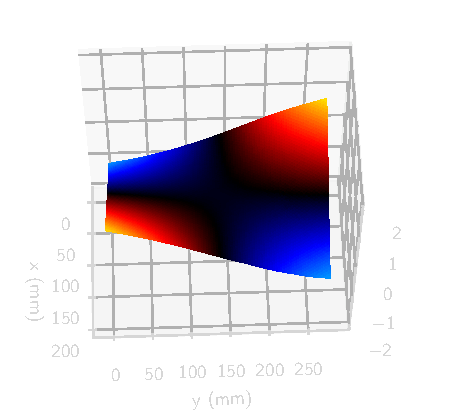
\includegraphics[width=27mm]{Plate/DS_n/1.pdf}}%
					&
					{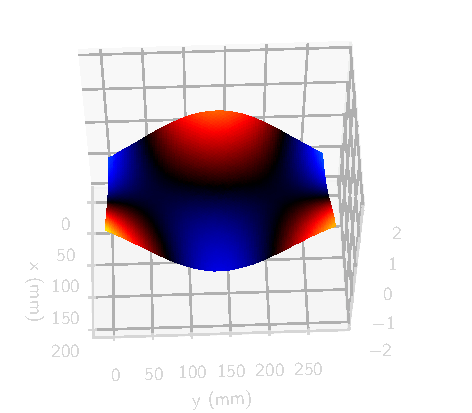
\includegraphics[width=27mm]{Plate/DS_n/3.pdf}}%
					\tabularnewline
					{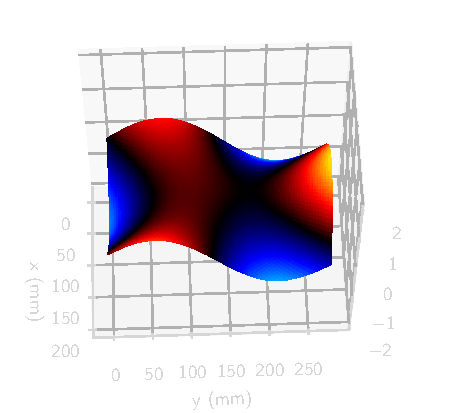
\includegraphics[width=27mm]{Plate/DS_n/5.pdf}}%
					&
					{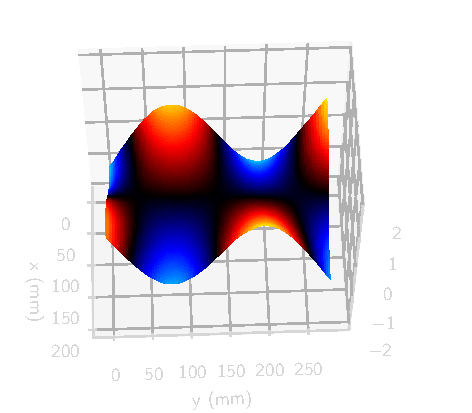
\includegraphics[width=27mm]{Plate/DS_n/8.pdf}}%
				\end{tabular}
			} ;
		}
		\visible<5>{
			\node at (-25mm, -40mm) {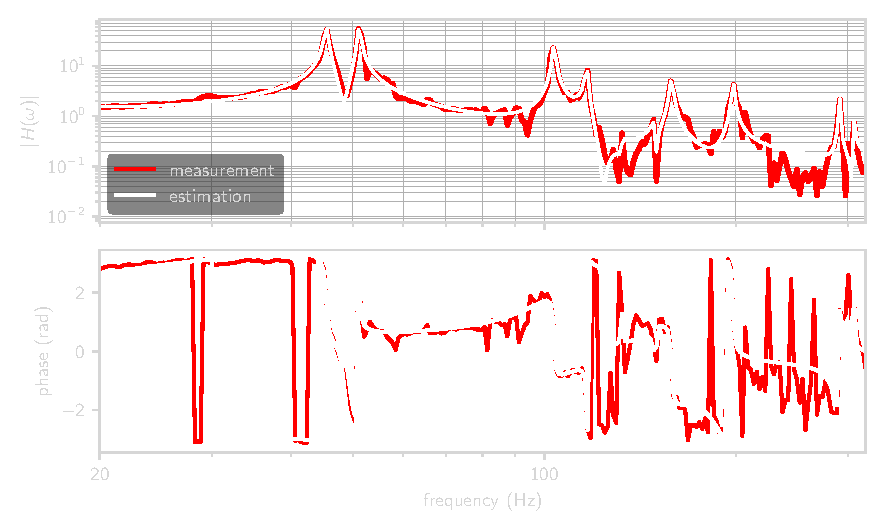
\includegraphics[width=60mm]{Plate/estimated_FRF.pdf}} ;
		}
		\visible<4>{
		\node at (-20mm,-33mm) {
			\movie[width=35mm]{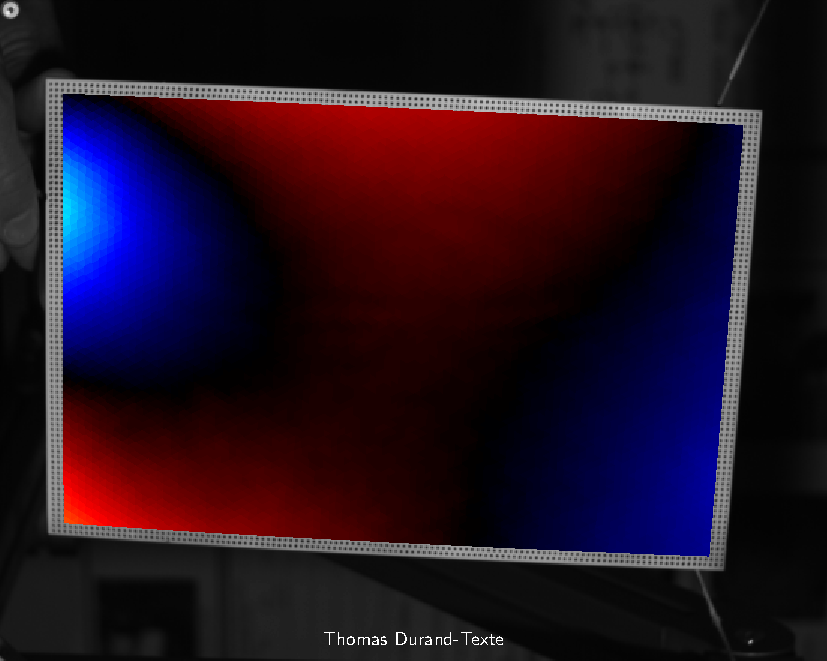
\includegraphics[width=35mm]{Plate/Movie_plate.pdf}}{Movie_plate.mp4}
		};
		}
		\visible<3,7->{
			\node at (-25mm, -35mm) { 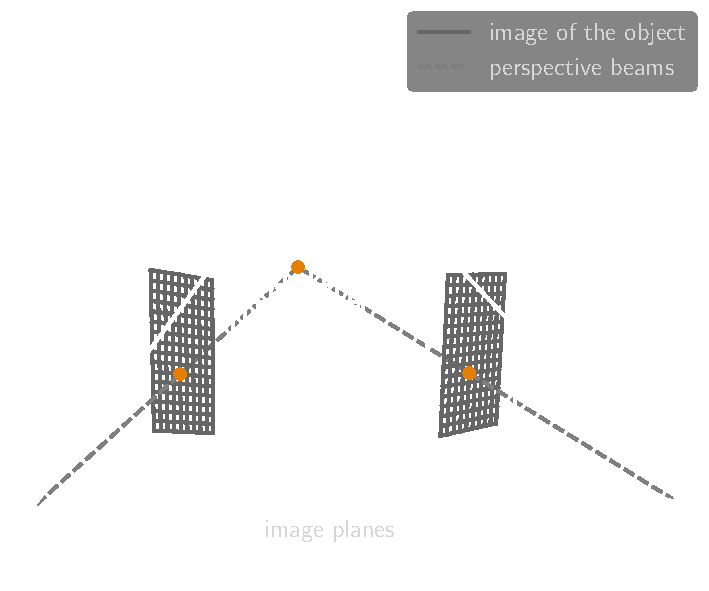
\includegraphics[width=55mm]{triangulation.pdf} } ;
		}
	
		\node at (-30mm, 13mm) { \movie[loop,width=30mm]{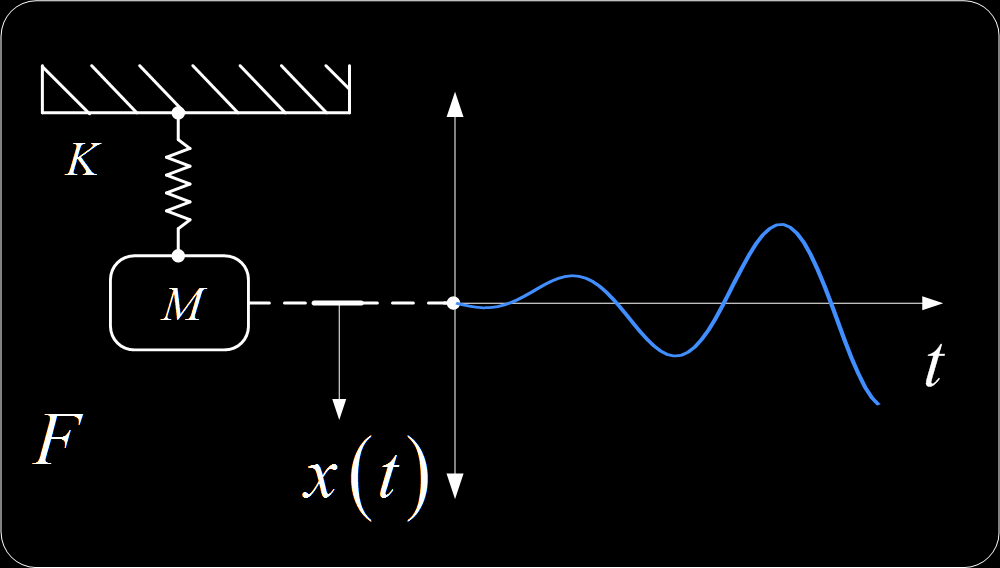
\includegraphics[width=30mm]{vib/Mass_Spring_dark-0.png}}{mass_spring.mp4} } ;
		\visible<2->{
			\node at (40mm,-12.5mm) {
\includegraphics[width=15mm]{electroac/loudspeaker.pdf}} ;
		}

	}
	\end{tikzpicture}
\end{frame}


\section{{\alert{Pourquoi} une nouvelle formation~?\\Dans \alert{quel but}~?}}

\begin{frame}[t]
	\vspace{0mm}
	\begin{tikzpicture}
		\draw[black] (0,0) rectangle (\textwidth,\textheight) ;
		\only<1-4>{
			\node[anchor=center] at (0.5\textwidth, 0.5\textheight) {\fontfamily{qcr}\fontsize{100pt}{20pt}\selectfont \color{myOrng}?} ;
			\node at (0.5\textwidth, 0.4\textheight) {
\includegraphics[width=6mm]{Logo_OpenClassrooms.png}} ;
			% \node[anchor=center] at (0.5\textwidth, 0.5\textheight) {\fontfamily{lmtt}\fontsize{100pt}{20pt}\selectfont \color{myOrng}?} ;
			% \node[anchor=center] at (0.5\textwidth, 0.5\textheight) {\fontfamily{phv}\fontsize{100pt}{20pt}\selectfont \color{myOrng}?} ;
			% \node[anchor=center] at (0.5\textwidth, 0.5\textheight) {\fontfamily{qhv}\fontsize{100pt}{20pt}\selectfont \color{myOrng}?} ;
			% \node at (0.495\textwidth, 0.38\textheight) {
\includegraphics[width=6mm]{Logo_OpenClassrooms.png}} ;
		}
		\only<5->{
			\node[anchor=center] at (0.5\textwidth, 0.5\textheight) {
\includegraphics[width=15mm]{Logo_OpenClassrooms.png}} ;
		}
		\only<6>{
			\node[box_style0, text width=30mm] at (0.5\textwidth,0.2\textheight) {{\color{myOrng}Création\\micro-entreprise\\(freelance)}} ;
			\node[anchor=center] at (0.2\textwidth,0.2\textheight) {
\includegraphics[height=12mm]{divers/creation.jpg}} ;
		}
		\visible<2->{
			\node[box_style0, text width=30mm] at (0.5\textwidth,0.8\textheight) {Plaisir d'\alert{apprendre}} ;
			\node[anchor=center] at (0.85\textwidth,0.8\textheight) {
\includegraphics[height=16mm]{divers/1213457-fond-tableau-noir-avec-elements-scolaires-vectoriel.jpg}} ;
		}
		\visible<3->{
			\node[box_style0, text width=30mm] at (0.2\textwidth,0.5\textheight) {Élargir mon champ de \alert{compétences}} ;
			% \node[anchor=center] at (0.12\textwidth,0.35\textheight) {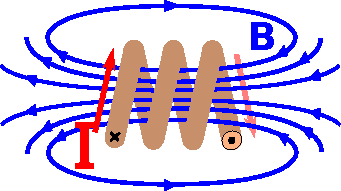
\includegraphics[width=15mm]{divers/magnetfeld_einer_spule_02.pdf}} ;
			% \node[anchor=center] at (0.2\textwidth,0.35\textheight) {
\includegraphics[width=15mm]{divers/Prismatic-Cloud-Gears-2.pdf}} ;
			\node[anchor=center] at (0.2\textwidth,0.7\textheight) {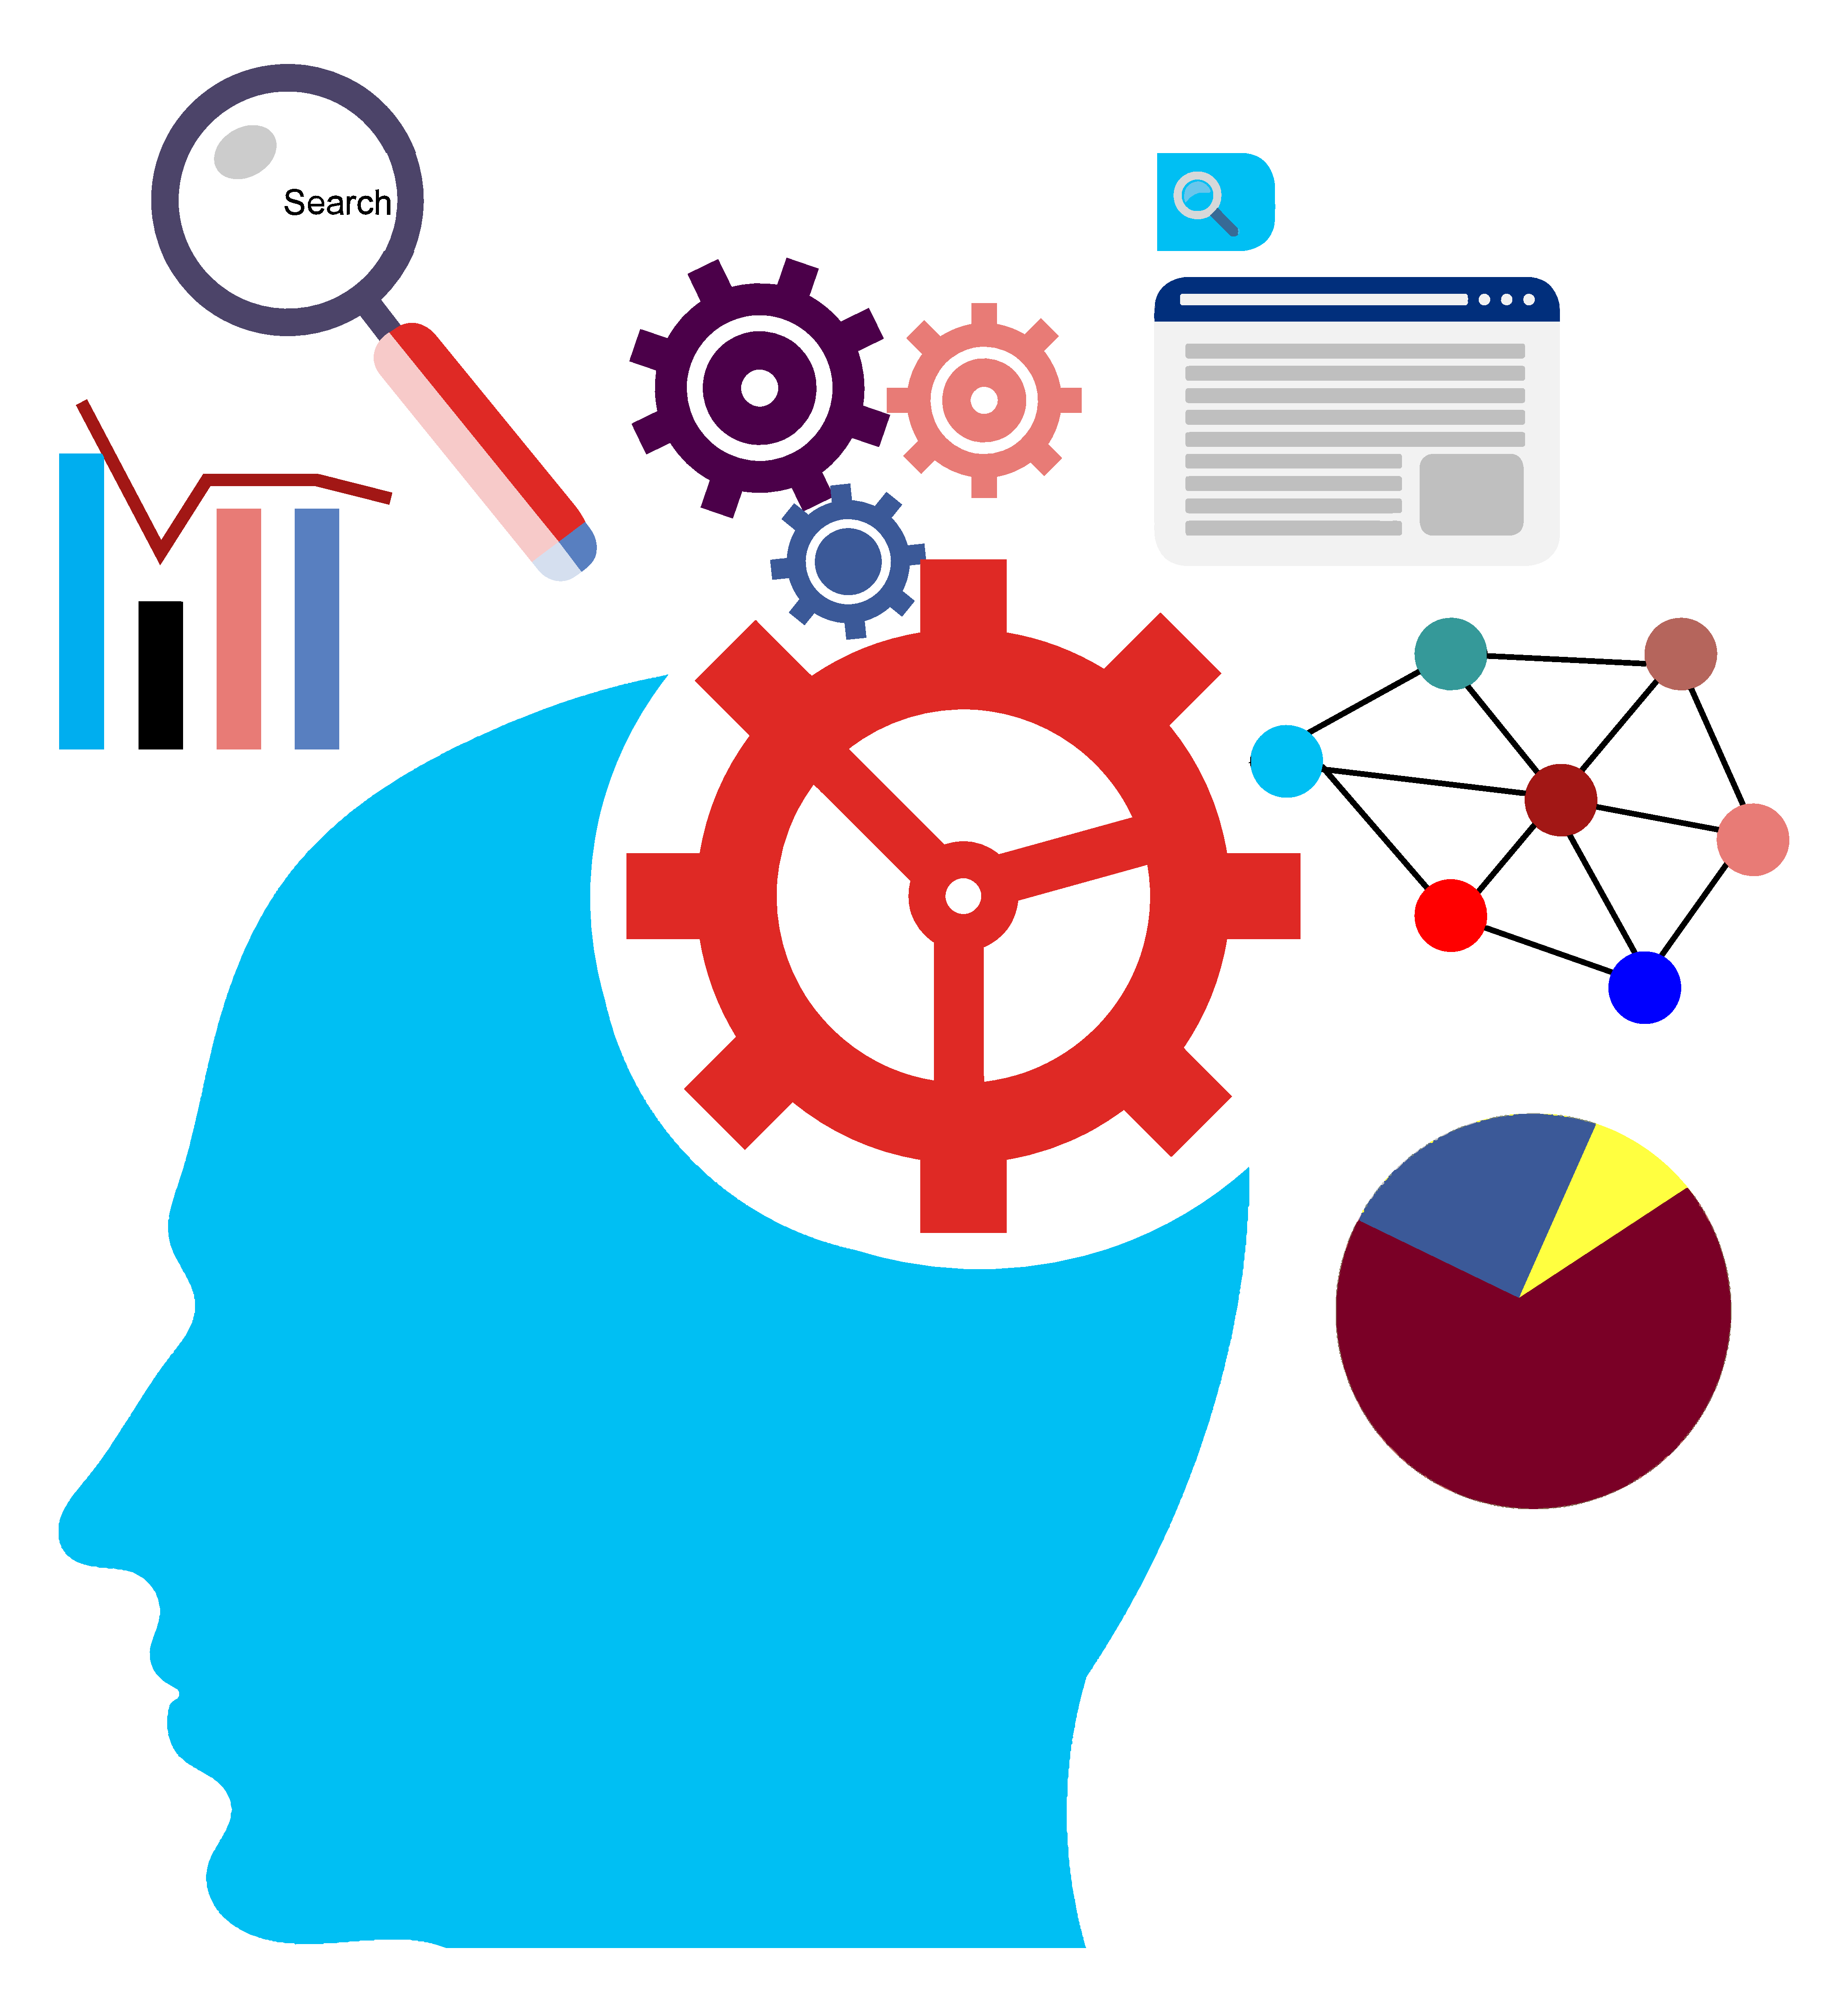
\includegraphics[width=20mm]{divers/Digital-Marketing.pdf}} ;
		}
		\visible<4->{
			\node[box_style0, text width=30mm] at (0.8\textwidth,0.5\textheight) {{Accéder à\\\vspace{0mm}de nouvelles \alert{opportunités}}} ;
			\node[anchor=center] at (0.85\textwidth,0.35\textheight) { 
\includegraphics[width=20mm]{divers/changechance.jpg} } ;
		}
	\end{tikzpicture}
\end{frame}



\section{Pourquoi OpenClassrooms~?}

\begin{frame}[t]
	\vspace{0mm}
	\begin{tikzpicture}
		\draw[black] (0,0) rectangle (\textwidth,\textheight) ;
		\begin{scope}[xshift=0.5\textwidth, yshift=0.5\textheight]
			\node[anchor=center] at (0, 0) {
\includegraphics[width=15mm]{Logo_OpenClassrooms.png}} ;
			
			\draw (90:\Rfive) node (E1) {} ;
			\draw (90-360/5:\Rfive) node (E2) {} ; 
			\draw (90-2*360/5:\Rfive) node (E3) {} ;
			\draw (90-3*360/5:\Rfive) node (E4) {} ; 
			\draw (90-4*360/5:\Rfive) node (E5) {} ; 

			
			\visible<3->{\draw[myarrow] (E1.center) arc (90:90-52:\Rfive ) ;}
			\visible<4->{\draw[myarrow] (E2.center) arc (90-360/5:90-360/5-52:\Rfive ) ;}
			\visible<5->{\draw[myarrow] (E3.center) arc (90-2*360/5:90-2*360/5-52:\Rfive ) ;}
			\visible<6->{\draw[myarrow] (E4.center) arc (90-3*360/5:90-3*360/5-52:\Rfive ) ;}
			\visible<7->{\draw[myarrow] (E5.center) arc (90-4*360/5:90-4*360/5-52:\Rfive ) ;}
			
			\visible<2->{
			\filldraw[fill=clrE1,clrE1] (E1.center) circle (\RelemFive) ;
			\node[circle_Five, text=black, text width=30mm] at (E1.center) {{Formations\\reconnues}} ; 
			\node[anchor=center] at (0.16\textwidth,0.37\textheight) {
\includegraphics[width=12mm]{divers/Merlin2525-Approved-Business-Stamp-1.pdf}} ;
			}
			
			\visible<3->{
			\filldraw[fill=clrE2,clrE2] (E2.center) circle (\RelemFive) ;
			\node[circle_Five, text=black] at (E2.center) {{Mentorat 45~min/sem.}} ;
			\node at (0.4\textwidth,0.32\textheight) {
\includegraphics[width=25mm]{divers/Mentorat.png}} ; 
			}
			
			\visible<4->{
			\filldraw[fill=clrE3,clrE3] (E3.center) circle (\RelemFive) ;
			\node[circle_Five,text=black] at (E3.center) {Accès à une communauté} ; 
			\node at (40mm,-25mm) {
\includegraphics[width=20mm]{Slack_logo_white.pdf}} ; 
			}

			\visible<5->{
			\filldraw[fill=clrE4,clrE4] (E4.center) circle (\RelemFive) ;
			\node[circle_Five,text=black] at (E4.center) {En distanciel} ;
			\node at (-44mm,-25mm) {
\includegraphics[width=20mm]{divers/icon-computer.pdf}} ; 
			}
			
			\visible<6->{
				\filldraw[fill=clrE5,clrE5] (E5.center) circle (\RelemFive) ;
				\node[circle_Five,text=black] at (E5.center) {{Apprentissage par projets}} ; 
				\node at (-40mm,30mm) {
\includegraphics[width=20mm]{divers/project-time.pdf}} ; 
			}
		\end{scope}
	\end{tikzpicture}
\end{frame}


\section{Les projets}

\begin{frame}[t]
	\vspace{0mm}
	\begin{tikzpicture}
		\draw[black] (0,0) rectangle (\textwidth,\textheight) ;
		
		\node at (0.5\textwidth-40mm,0.5\textheight+30mm) {
\includegraphics[width=20mm]{divers/project-time.pdf}} ; 
		\node at (0.5\textwidth,0.9\textheight) {\large \color{myOrng} \textbf{Projets}} ;
		
		\visible<3->{\filldraw[black!75, rounded corners] ( 0.2875\textwidth, 0.06\textwidth ) rectangle (0.7125\textwidth,0.85\textheight) ;}

		\only<2>{\node[box_style0, text width=0.2\textwidth] at (0.15\textwidth,0.65\textheight) {1} ;}
		\only<3-4>{
			\node[box_style0, myOrng, fill=black!75, font=\bfseries, text width=0.2\textwidth] at (0.15\textwidth,0.65\textheight) {1} ;
			\node[text width=0.4\textwidth, text centered, font=\bfseries] at (0.5\textwidth,0.78\textheight) {{Concevez une application\\au service de la santé publique}} ;
			\node[text width=0.41\textwidth, anchor=north west] at (0.27\textwidth,0.75\textheight) {
				\begin{itemize}
					\item[$\bullet$] \alert{Gestion} de \alert{données} incomplètes
					\item[$\bullet$] \alert{Analyse statistique} uni/multivariée
					\item[$\bullet$] \alert{Communication} sur les résultats
					% \item[$\bullet$] motivation : prise en main / découverte
				\end{itemize}
			} ;
		}

		
		\only<2-4>{\node[box_style0, text width=0.2\textwidth] at (0.15\textwidth,0.56\textheight) {2} ;}
		\only<5-6>{
			\node[box_style0, myOrng, fill=black!75, font=\bfseries, text width=0.2\textwidth] at (0.15\textwidth,0.56\textheight) {2} ;
			\node[text width=0.4\textwidth, text centered, font=\bfseries] at (0.5\textwidth,0.78\textheight) {{Anticipez les besoins\\en consommation de bâtiments}} ;
			\node[text width=0.41\textwidth, anchor=north west] at (0.27\textwidth,0.75\textheight) {
				\begin{itemize}
					\item[$\bullet$] Mise en place d'un \alert{modèle} d'apprentissage \alert{supervisé}
					\item[$\bullet$] \alert{Transformation} des \alert{variables} pertinentes
					\item[$\bullet$] \alert{Adaptation} des hyperparamètres
					\item[$\bullet$] \alert{Évaluation} des \alert{performances} du modèle
				\end{itemize}
			} ;
		}


		\only<2-6>{\node[box_style0, text width=0.2\textwidth] at (0.15\textwidth,0.47\textheight) {3} ;}
		\only<7-8>{
			\node[box_style0, myOrng, fill=black!75, font=\bfseries, text width=0.2\textwidth] at (0.15\textwidth,0.47\textheight) {3} ;
			\node[text width=0.4\textwidth, text centered, font=\bfseries] at (0.5\textwidth,0.78\textheight) {{Segmentez des clients\\d'un site e-commerce}} ;
			\node[text width=0.41\textwidth, anchor=north west] at (0.27\textwidth,0.75\textheight) {
				\begin{itemize}
					\item[$\bullet$] Mise en place d'un \alert{modèle} d'apprentissage \alert{non-supervisé}
					\item[$\bullet$] \alert{Transformation} des \alert{variables} pertinentes
					\item[$\bullet$] \alert{Adaptation} des hyperparamètres
					\item[$\bullet$] \alert{Évaluation} des \alert{performances} du modèle
				\end{itemize}
			} ;
		}

		\only<2-8>{\node[box_style0, text width=0.2\textwidth] at (0.15\textwidth,0.38\textheight) {4} ;}
		\only<9-10>{
			\node[box_style0, myOrng, fill=black!75, font=\bfseries, text width=0.2\textwidth] at (0.15\textwidth,0.38\textheight) {4} ;
			\node[text width=0.4\textwidth, text centered, font=\bfseries] at (0.5\textwidth,0.78\textheight) {{Catégorisez automatiquement\\des questions}} ;
			\node[text width=0.41\textwidth, anchor=north west] at (0.27\textwidth,0.75\textheight) {
				\begin{itemize}
					\item[$\bullet$] \alert{Gestion} de \alert{données} à grandes dimensions
					\item[$\bullet$] \alert{Prétraitement} des \alert{données non structurées}
					\item[$\bullet$] Mise en \oe{}uvre des techniques de \alert{réduction de dimension}
					\item[$\bullet$] Mise en \oe{}uvre des techniques d'\alert{extraction de features} pour des données non structurées
				\end{itemize}
			} ;
		}

		\only<2-10>{\node[box_style0, text width=0.2\textwidth] at (0.15\textwidth,0.29\textheight) {5} ;}
		\only<11-12>{
			\node[box_style0, myOrng, fill=black!75, font=\bfseries, text width=0.2\textwidth] at (0.15\textwidth,0.29\textheight) {5} ;
			\node[text width=0.4\textwidth, text centered, font=\bfseries] at (0.5\textwidth,0.78\textheight) {{Classez des images à l'aide\\d'algorithmes de Deep Learning}} ;
			\node[text width=0.41\textwidth, anchor=north west] at (0.27\textwidth,0.75\textheight) {
				\begin{itemize}
					\item[$\bullet$] Mise en place d'un \alert{modèle} de \alert{Deep Learning}
					\item[$\bullet$] \alert{Sélection} d'un modèle d'apprentissage \alert{adapté}
					\item[$\bullet$] \alert{Transformation} des \alert{variables} pertinentes
					\item[$\bullet$] \alert{Évaluation} des \alert{performances} du modèle
				\end{itemize}
			} ;
		}

		\only<2-12>{\node[box_style0, text width=0.2\textwidth] at (0.15\textwidth,0.20\textheight) {6} ;}
		\only<13-14>{
			\node[box_style0, myOrng, fill=black!75, font=\bfseries, text width=0.2\textwidth] at (0.15\textwidth,0.20\textheight) {6} ;
			\node[text width=0.4\textwidth, text centered, font=\bfseries] at (0.5\textwidth,0.78\textheight) {{Développez une preuve de concept}} ;
			\node[text width=0.41\textwidth, anchor=north west] at (0.27\textwidth,0.75\textheight) {
				\begin{itemize}
					\item[$\bullet$] \alert{Réalisation} d'une \alert{veille} sur les évolutions de la \alert{Data Science}
					\item[$\bullet$] \alert{Développement} d'une preuve de concept
					\item[$\bullet$] \alert{Identification} des méthodes "\alert{état de l'art}"
					\item[$\bullet$] \alert{Identification} des \alert{sources} d'informations \alert{fiables} et \alert{pertinentes}
				\end{itemize}
			} ;
		}

		\only<2-14>{\node[box_style0, text width=0.2\textwidth] at (0.15\textwidth,0.11\textheight) {7} ;}
		\only<15-16>{
			\node[box_style0, myOrng, fill=black!75, font=\bfseries, text width=0.2\textwidth] at (0.15\textwidth,0.11\textheight) {7} ;
			\node[text width=0.4\textwidth, text centered, font=\bfseries] at (0.5\textwidth,0.78\textheight) {{Participez à une\\compétition Kaggle~!}} ;
			\node[text width=0.41\textwidth, anchor=north west] at (0.27\textwidth,0.75\textheight) {
				\begin{itemize}
					\item[$\bullet$] \alert{Présentation} de code aux standards \alert{PEP 8}
					\item[$\bullet$] \alert{Gestion} des \alert{versions de code}% pour assurer l'\alert{intégration du modèle}
					\item[$\bullet$] \alert{Rédaction} d'une \alert{note méthodologique}% afin de communiquer sa démarche de modélisation
					\item[$\bullet$] \alert{Enrichissement} des \alert{réalisations} d'autres membres de la \alert{communauté} de professionnels
				\end{itemize}
			} ;
		}

		% Anticipez les besoins en consommation de bâtiments
		% Évaluer les performances d'un modèle d'apprentissage supervisé
		% Transformer les variables pertinentes d'un modèle d'apprentissage supervisé
		% Adapter les hyperparamètres d'un algorithme d'apprentissage supervisé afin de l'améliorer
		% Mettre en place le modèle d'apprentissage supervisé adapté au problème métier

		% Segmentez des clients d'un site e-commerce
		% Mettre en place le modèle d'apprentissage non supervisé adapté au problème métier
		% Transformer les variables pertinentes d'un modèle d'apprentissage non supervisé
		% Évaluer les performances d'un modèle d'apprentissage non supervisé
		% Adapter les hyperparamètres d'un algorithme non supervisé afin de l'améliorer

		% Catégorisez automatiquement des questions
		% Représenter graphiquement des données à grandes dimensions
		% Prétraiter des données non structurées pour obtenir un jeu de données exploitable
		% Mettre en œuvre des techniques de réduction de dimension
		% Mettre en œuvre des techniques d'extraction de features pour des données non structurées

		% Classez des images à l'aide d'algorithmes de Deep Learning
		% Transformer les variables pertinentes d'un modèle de Deep Learning
		% Adapter les paramètres d'un modèle de Deep Learning afin de l'améliorer
		% Mettre en place un modèle de Deep Learning
		% Sélectionner un modèle d'apprentissage Deep Learning adapté à une problèmatique métier
		% Évaluer les performances d'un modèle de Deep Learning

		% Développez une preuve de concept (PoC)
		% Réaliser une veille sur les évolutions de la Data Science
		% Développer une preuve de concept pour résoudre un problème de Data science
		% Identifier les méthodes "état de l'art" pour résoudre un problème de Data science
		% Identifier des sources d'informations fiables et pertinentes

		% Participez à une compétition Kaggle !
		% Présenter son code aux standards PEP 8
		% Utiliser un logiciel de version de code pour assurer l'intégration du modèle
		% Rédiger une note méthodologique afin de communiquer sa démarche de modélisation
		% Enrichir les réalisations d'autres membres de la communauté de professionnels

		\visible<4->{\node[box_style0, text width=0.2\textwidth] at (0.85\textwidth,0.9\textheight) {Santé} ;}
		\visible<6->{\node[box_style0, text width=0.2\textwidth] at (0.85\textwidth,0.8\textheight) {Énergie} ;}
		\visible<8->{\node[box_style0, text width=0.2\textwidth] at (0.85\textwidth,0.7\textheight) {Segmenter} ;}
		\visible<10->{\node[box_style0, text width=0.2\textwidth] at (0.85\textwidth,0.6\textheight) {Catégoriser} ;}
		\visible<12->{\node[box_style0, text width=0.2\textwidth] at (0.85\textwidth,0.5\textheight) {Classer/images} ;}
		\visible<14->{\node[box_style0, text width=0.2\textwidth] at (0.85\textwidth,0.4\textheight) {PoC} ;}
		\visible<16->{\node[box_style0, text width=0.2\textwidth] at (0.85\textwidth,0.3\textheight) {Kaggle} ;}


	\end{tikzpicture}
\end{frame}


\begin{frame}[t]
	\vspace{0mm}
	\begin{tikzpicture}
		\draw[black] (0,0) rectangle (\textwidth,\textheight) ;
		
		\node at (0.5\textwidth-40mm,0.5\textheight+30mm) {
\includegraphics[width=20mm]{divers/project-time.pdf}} ; 
		\node at (0.5\textwidth,0.9\textheight) {\large \color{myOrng} \textbf{Projets}} ;
		
		\visible<2->{
		\node at (0.15\textwidth,0.60\textheight) { Les plus \textcolor{green}{motivants}} ;
		}

		\visible<4->{
		\node at (0.5\textwidth,0.60\textheight) { \textcolor{red}{Difficiles} (à priori) } ;
		}

		\only<-2>{
			\node[box_style0, text width=0.2\textwidth] at (0.85\textwidth,0.9\textheight) {Santé} ;
			\node[box_style0, text width=0.2\textwidth] at (0.85\textwidth,0.8\textheight) {Énergie} ;
			\node[box_style0, text width=0.2\textwidth] at (0.85\textwidth,0.5\textheight) {Classer/images} ;
		}
		\only<3->{\node[box_style0, text width=0.2\textwidth] at (0.15\textwidth,0.5\textheight) {Santé} ;
			\node[box_style0, text width=0.2\textwidth] at (0.15\textwidth,0.4\textheight) {Énergie} ;
			\node[box_style0, text width=0.2\textwidth] at (0.15\textwidth,0.3\textheight) {Classer/images} ;
		}

		\only<-4>{
			\node[box_style0, text width=0.2\textwidth] at (0.85\textwidth,0.7\textheight) {Segmenter} ;
			\node[box_style0, text width=0.2\textwidth] at (0.85\textwidth,0.6\textheight) {Catégoriser} ;
			\node[box_style0, text width=0.2\textwidth] at (0.85\textwidth,0.3\textheight) {Kaggle} ;
		}

		\only<5->{
			\node[box_style0, text width=0.2\textwidth] at (0.5\textwidth,0.5\textheight) {Segmenter} ;
			\node[box_style0, text width=0.2\textwidth] at (0.5\textwidth,0.4\textheight) {Catégoriser} ;
			\node[box_style0, text width=0.2\textwidth] at (0.5\textwidth,0.3\textheight) {Kaggle} ;
		}
		
		\only<-5>{\node[box_style0, text width=0.2\textwidth] at (0.85\textwidth,0.4\textheight) {PoC} ;}
		\only<6>{
			\node[box_style0, text width=0.2\textwidth] at (0.85\textwidth,0.5\textheight) {PoC} ;
			\node[text centered] at (0.85\textwidth,0.6\textheight) { \Huge ? } ;
		}

	\end{tikzpicture}
\end{frame}




% \subsection{Les plus motivants}
% \begin{frame}
% 	\shdd{Les projets  les plus \alert{motivants}~:}
	
% 	\vspace{6mm}
% 	\def\arraystretch{2}%  1 is the default, change whatever you need
% 	\begin{tabular}{>{\centering}m{50mm}c>{\centering}m{40mm}}
% 		\shdng{0}{1}{2-}{Concevez une application au service de la santé publique}
% 		&
% 		\shdng{0}{1}{2-}{\Huge $\rightarrow$}
% 		&
% 		\shdng{0}{1}{2-}{alimentation, prie en main des outils}
% 		\tabularnewline
% 		\shdng{-1}{2}{3-}{Anticipez les besoins en consommation de bâtiments}
% 		&
% 		\shdng{-1}{2}{3-}{\Huge $\rightarrow$}
% 		&
% 		\shdng{-1}{2}{3-}{modélisation, énergie}
% 		\tabularnewline
% 		\shdng{-2}{3}{0}{Classez des images à l'aide d'algorithmes de Deep Learning}
% 		&
% 		\shdng{-2}{3}{0}{\Huge $\rightarrow$}
% 		&
% 		\shdng{-2}{3}{0}{traitement d'images, (Deep learning?)}
% 	\end{tabular}
% \end{frame}

% \subsection{Les plus difficiles à priori}

% \begin{frame}
% 	\shdd{Les projets  les plus \alert{difficiles} à priori~:}
	
% 	\vspace{6mm}
% 	\def\arraystretch{2}%  1 is the default, change whatever you need
% 	\begin{tabular}{>{\centering}m{50mm}c>{\centering}m{40mm}}
% 		\shdng{0}{1}{2-}{Segmentez des clients d'un site e-commerce}
% 		&
% 		\shdng{0}{1}{2-}{\Huge $\rightarrow$}
% 		&
% 		\shdng{0}{1}{2-}{plus éloigné de mes compétences}
% 		\tabularnewline
% 		\shdng{-1}{2}{3-}{Catégorisez automatiquement des questions}
% 		&
% 		\shdng{-1}{2}{3-}{\Huge $\rightarrow$}
% 		&
% 		\shdng{-1}{2}{3-}{plus éloigné de mes compétences}
% 		\tabularnewline
% 		\shdng{-2}{3}{0}{Participez à une compétition Kaggle !}
% 		&
% 		\shdng{-2}{3}{0}{\Huge $\rightarrow$}
% 		&
% 		\shdng{-2}{3}{0}{compétition}
% 	\end{tabular}
% \end{frame}

\section{Planification}
\begin{frame}[t]
	\vspace{6mm}
	\shdd{Notebook pour estimer les \alert{dates prévisionnelles} de soutenances~:}

	\vfill
	\only<1>{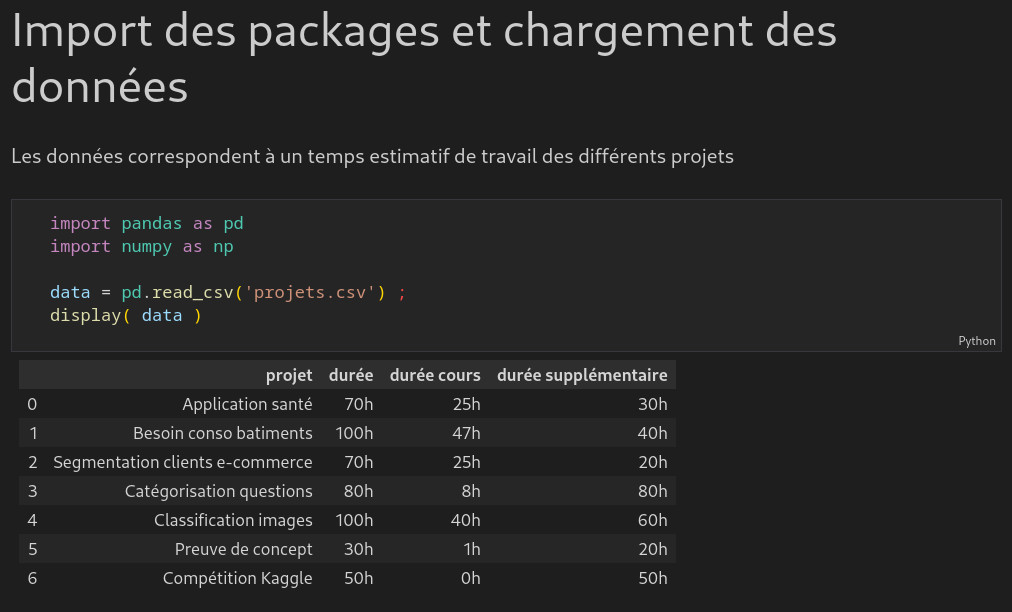
\includegraphics[width=110mm]{dates/cell-1.jpg}}%
	\only<2>{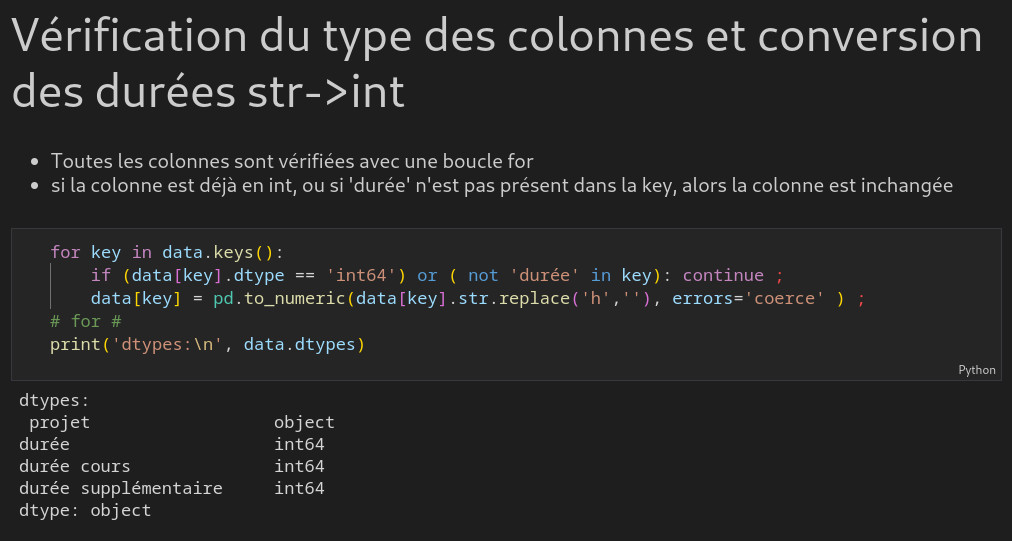
\includegraphics[width=110mm]{dates/cell-2.jpg}}%
	\only<3>{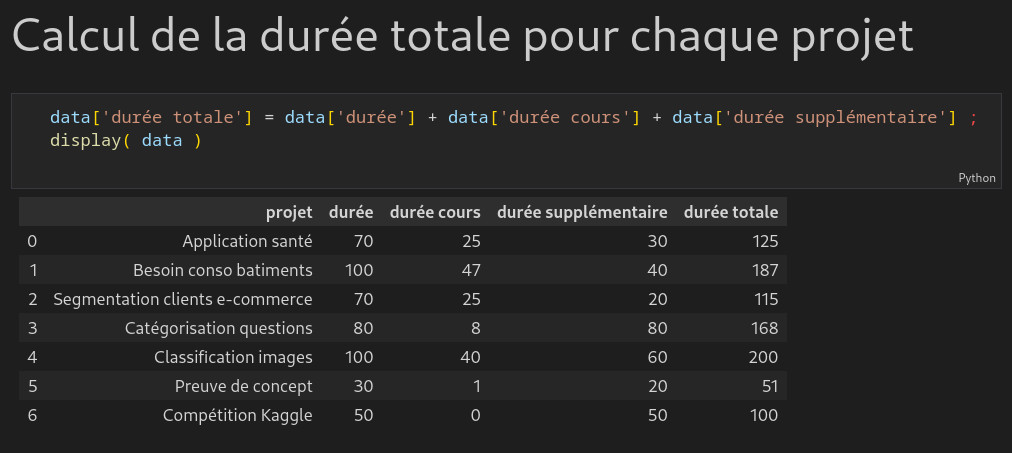
\includegraphics[width=110mm]{dates/cell-3.jpg}}%
	\only<4>{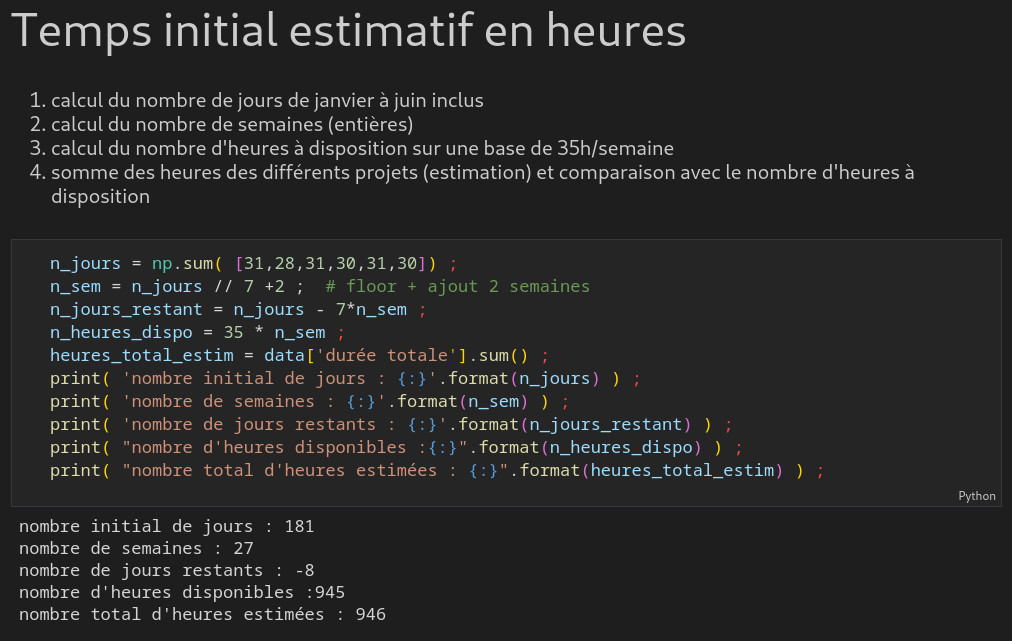
\includegraphics[width=110mm]{dates/cell-4.jpg}}%
	\only<5>{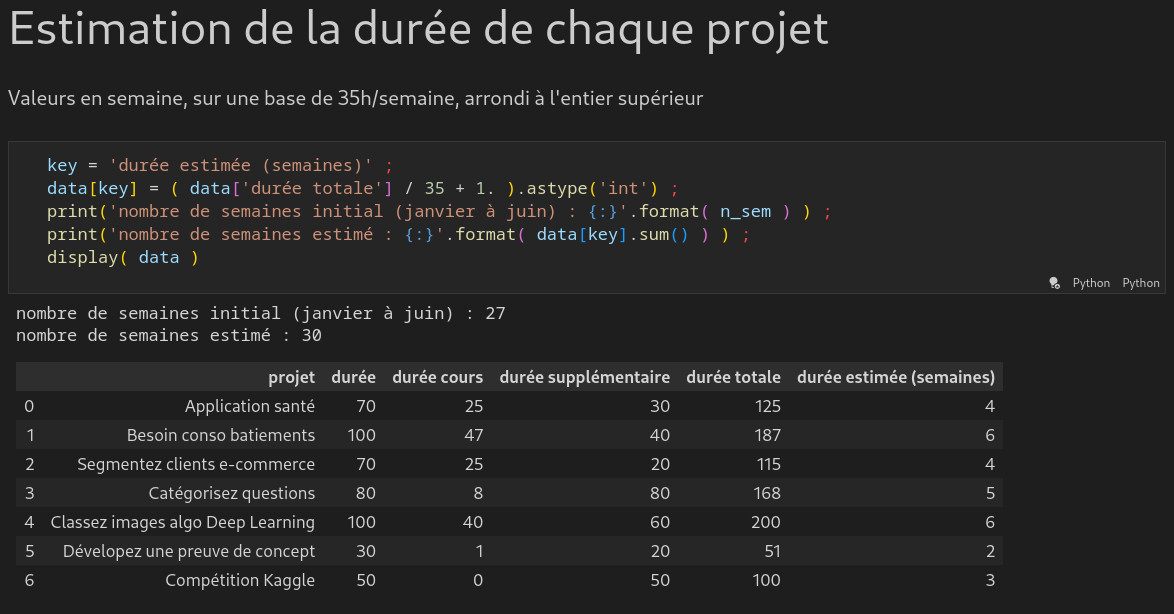
\includegraphics[width=110mm]{dates/cell-5.jpg}}%
	\only<6>{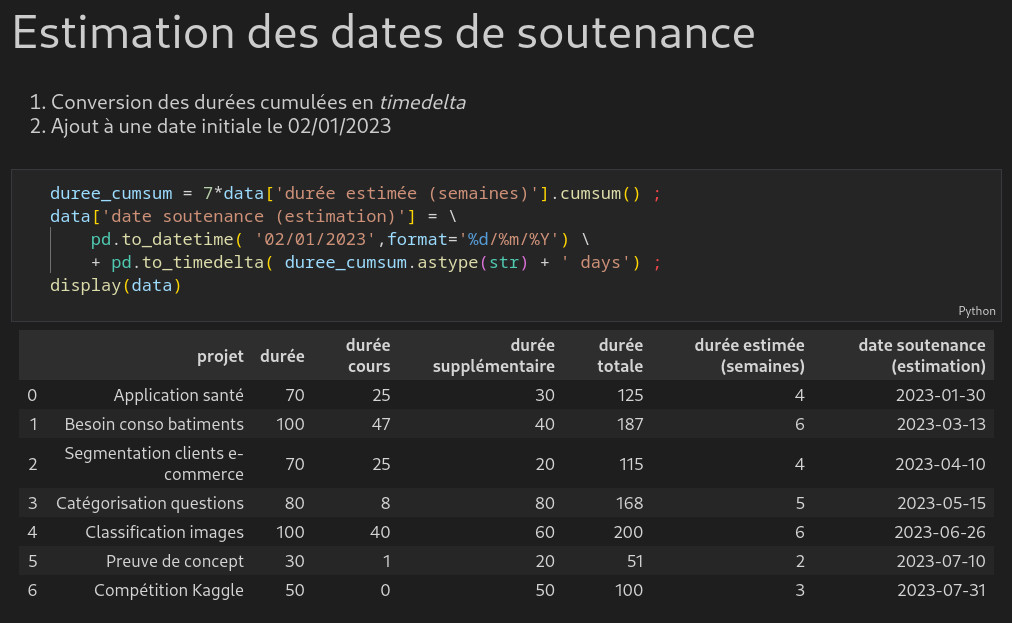
\includegraphics[width=110mm]{dates/cell-6.jpg}}%
	\only<7->{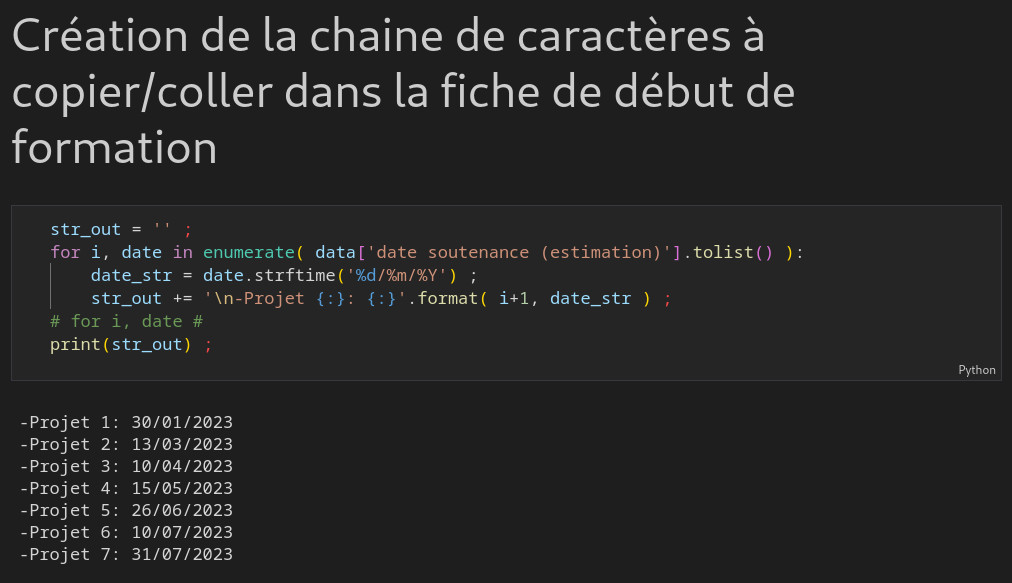
\includegraphics[width=110mm]{dates/cell-7.jpg}
	\visible<8>{Date limite de fin de formation : 21/08/2023 }
	}%
	\vfill

\end{frame}

\section{Quelques bonnes pratiques}

\begin{frame}[t]
	\vspace{0mm}
	\begin{tikzpicture}
		\draw[black] (0,0) rectangle (\textwidth,\textheight) ;
		
		\visible<2->{\node[box_style0, text width=38mm] (A) at (0.7\textwidth, 0.8\textheight) {{Calendrier\\\vspace{-1mm}(dates des jalons)}} ;}
		\visible<3->{\node[box_style0, text width=38mm] (B) at (0.7\textwidth, 0.6\textheight) {{Technique POMODORO\\\vspace{-1mm}(limite la fatigue)}} ;}
		\visible<4->{\node[box_style0, text width=38mm] (C) at (0.7\textwidth, 0.4\textheight) {{Préparation\\\vspace{-1mm}sessions mentorat}} ;}
		\visible<5->{\node[box_style0, text width=38mm] (D) at (0.7\textwidth, 0.2\textheight) {{Éviter de rester bloqué\\\vspace{-1mm}(avancer sur autre chose)}} ;}
		
		\only<1-9>{
			\node at (0.2\textwidth,0.5\textheight) {
\includegraphics[width=30mm]{divers/smiley_ko.pdf}} ;
			\only<2->{	\draw[myarrow] (0.3\textwidth, 0.6\textheight) -- (A.west) ; }
			\only<3->{	\draw[myarrow] (0.33\textwidth, 0.52\textheight) -- (B.west) ; }
			\only<4->{	\draw[myarrow] (0.33\textwidth, 0.48\textheight) -- (C.west) ; }
			\only<5->{	\draw[myarrow] (0.3\textwidth, 0.4\textheight) -- (D.west) ; }
		}

		\only<6->{ \node[green, right=of A.east, xshift=-7mm] {\huge \checkmark} ; }
		\only<7->{ \node[green, right=of B.east, xshift=-7mm] {\huge \checkmark} ; }
		\only<8->{ \node[green, right=of C.east, xshift=-7mm] {\huge \checkmark} ; }
		\only<9->{ \node[green, right=of D.east, xshift=-7mm] {\huge \checkmark} ; }
		
			
		\only<10->{
			\node at (0.2\textwidth,0.5\textheight) {
\includegraphics[width=30mm]{divers/smiley_ok.pdf}} ;
			% \node at (0.18\textwidth,0.525\textheight) {
\includegraphics[width=30mm]{divers/skotan-Thumbs-up-smiley.pdf}} ;
			\draw[myarrow, myOrng] (A.west) -- (0.3\textwidth, 0.6\textheight) ;
			\draw[myarrow, myOrng] (B.west) -- (0.33\textwidth, 0.52\textheight) ;
			\draw[myarrow, myOrng] (C.west) -- (0.33\textwidth, 0.48\textheight) ;
			\draw[myarrow, myOrng] (D.west) -- (0.3\textwidth, 0.4\textheight) ;
		}
	\end{tikzpicture}
\end{frame}



\section{Outils collaboratifs}

\begin{frame}[t]
	\vspace{0mm}
	\begin{tikzpicture}
		\draw[black] (0,0) rectangle (\textwidth,\textheight) ;

		\node[draw, rounded corners, anchor=north, text centered, text width=30mm] at (0.3\textwidth,0.8\textheight) {\large {Outils de\\\vspace{-1mm}\alert{communication}\\pour le \alert{Mentorat} }} ;
		% \node at (0.7\textwidth,0.8\textheight) {
\includegraphics[width=30mm]{divers/Business-Meeting-No-Background.pdf}} ;
		\node at (0.7\textwidth,0.72\textheight) {
\includegraphics[width=30mm]{divers/Computer-Handshake-1-by-Merlin2525.pdf}} ;

		\visible<2->{
		\node[box_style0, anchor=center] at (0.2\textwidth,0.47\textheight) {GitHub} ;
		\node[anchor=south] at (0.2\textwidth,0.17\textheight) {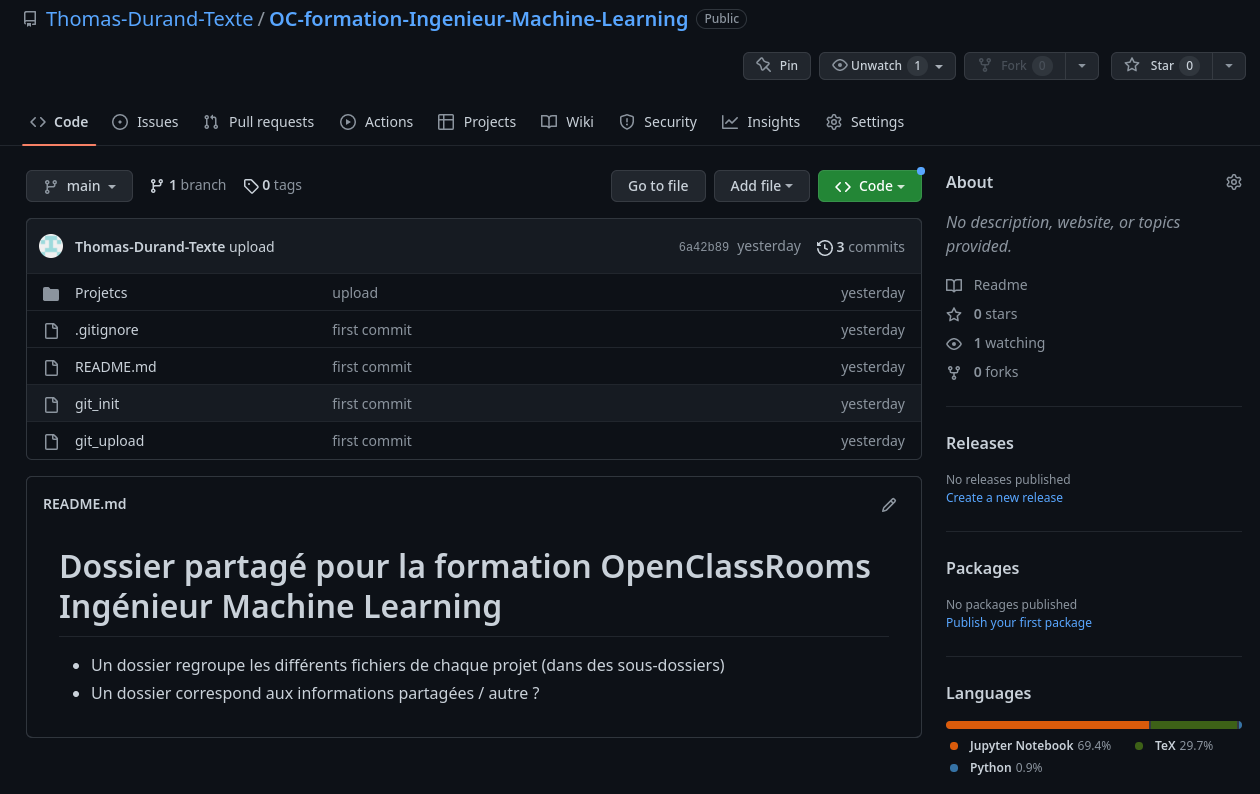
\includegraphics[width=0.3\textwidth]{GitHub.png}} ;
		}
		
		\visible<3->{
		\node[box_style0, anchor=center] at (0.5\textwidth,0.47\textheight) {E-mails} ;
		\node at (0.5\textwidth,0.5\textheight-18mm) {\includegraphics[height=10mm]{ divers/Email-8.pdf}} ;
		}

		\visible<4->{
		\node[box_style0, anchor=center] at (0.8\textwidth,0.47\textheight) {{OpenClassrooms}} ;
		\node at (0.8\textwidth,0.5\textheight-18mm) {\includegraphics[width=10mm]{Logo_OpenClassrooms.png	}} ;
		}
	\end{tikzpicture}
\end{frame}



\begin{frame}[t]
	\vspace{18mm}
	\begin{center}
		\Large \alert{Merci} pour votre \alert{attention}.
	\end{center}

	\vfill
	{\tiny
	\begin{center}
		\alert{Artworks}\\ \vspace{-2mm}
		\alert{\rule{40mm}{0.1mm}}
	\end{center}

	openclipart.org~:

	\begin{minipage}[t]{0.48\textwidth}
		\begin{itemize}
			\item[$\bullet$] loudspeaker by forestgreen
			\item[$\bullet$] Digital Marketing by GDJ
			\item[$\bullet$] Time Project by lbear
			\item[$\bullet$] Laptop Computer Icon by kael\_179
		\end{itemize}
	\end{minipage}
	\begin{minipage}[t]{0.48\textwidth}
		\begin{itemize}
			\item[$\bullet$] Approved Business Stamp 1, Computer Handshake 1 by Merlin2525
			\item[$\bullet$] Glossy Smiley Set 3 by Chrisdesign
			\item[$\bullet$] mail-8 by gezegen 
		\end{itemize}	
	\end{minipage}

	\vspace{3mm}
	
	\begin{minipage}[t]{0.48\textwidth}
		commons.wikimedia~: 
	\begin{itemize}
		\item[$\bullet$] Mass Spring System Resonance.gif by Guillermo Bossio 
	\end{itemize}
		Divers:
	\begin{itemize}
		\item[$\bullet$] Letting Go \& Leaning In - Turning Change Into Chance (pierretteraymond.com)
		\item[$\bullet$] dynamique-mag.com/article/etapes-cles-reussir-creation-entreprise.10007
	\end{itemize}

	\end{minipage}
	\begin{minipage}[t]{0.48\textwidth}
		Vecteezy:
		\begin{itemize}
			\item[$\bullet$] fond de tableau noir avec des éléments de fournitures scolaires by anuwat meereevee
			\item[$\bullet$] coach de vie pour la consultation, l'éducation, la motivation, la perspective de mentorat et l'auto-encadrement dans le modèle d'illustration plate de dessin animé dessiné à la main by denayunevz
		\end{itemize}
			
	\end{minipage}

	}% tiny

\end{frame}


% ------------------------------------------- %

\end{document}
